\documentclass{report}
\usepackage{graphicx}
\usepackage{fancyhdr}
\usepackage{hyperref}
\usepackage{subcaption}
\usepackage{adjustbox}
\usepackage [ a4paper , hmargin =1.2 in , bottom =1.5 in ] { geometry }
\hypersetup{
    colorlinks=true,
    linkcolor=blue,
    filecolor=magenta,      
    urlcolor=cyan,
}
\pagestyle{fancy}
\lhead{Python - Web Crawler}
\rhead{Saksham Rathi}
\fancyfoot[C]{Page Number: \thepage}
%\fancyhf[]{}
\bibliographystyle{plain}
\renewcommand\thesection{\arabic{section}}

\begin{document}

\title{CS 104 Project - Web Crawler}
\author{Saksham Rathi}
\maketitle

\tableofcontents

\clearpage

\section{Objective}
The python file \texttt{web\_crawler.py} implement a Web Crawler using Python and its libraries.
Another python file \texttt{customized\_web\_crawler.py} has some added customizations.


\section{Introduction to Web Crawler}
Web crawler is a computer program that is used to search and automatically index website
content and other information over the internet. These programs, or bots, are most commonly
used to create entries for a search engine index.

\section{Applications}
Some of the applications of a web crawler have been described in brief below:
\begin{itemize}
    \item \textbf{Search Engine Indexing}: They are used extensively by search engines like Google, Bing and Yahoo to discover web pages, index their content and update their search engine databases.
    \item \textbf{Security Assessments}: They can be utilized for security purposes, such as detecting vulnerabilities and security flaws on websites. They can help identify broken authentication mechanisms and insecure configurations.
    \item \textbf{Data Extraction}: They can be used to extract data from websites at scale. Examples include gathering pricing data, extracting news articles etc.
\end{itemize}

\section{A brief description of the code}
The base website link will be provided as a command line argument by the user. (Refer \ref{sec:Usage}) Now the python file will recursively find out all the unique referenced web links eith "href", "src" or some commonly used attributes with different tags. 


Recursion means, from the first input link given, it will be parsed. Let us suppose that the parsed HTML will give 10 links. Now, the code will visit these 10 links individually and then from each of these get more links.

These all links found will be written in a file. The recursion will apply only to internal links i.e. the links that belong to the same domain. Although the external links will be listed, but they will not be crawled on. The basic idea of the code has been taken from \cite{basic_idea}

\section{Working of the code}
The Python code uses different libraries for performing different tasks. The applications of these libraries are explained in the code using comments and also become clear as they get used later in the code.
The use of different variables including lists, dictionaries etc also has been explained, moreover desciptive names have been used for the ease of undestanding.
There is a main recursive function called scrape. It takes three parameters and then later recursively calls itself. It checks for different attributes in the HTML source file and then updates the dictionaries accordingly. If it finds that the link is internal and has not been called before, then it recursively calls the function on that link.
The code also breaks the terminal arguments and then performs its work. If the output file is given as an argument then the result is printed in that file with a legible syntax to allow the users to understand the output. If an output file is not present, then the output is printed on the terminal. The file \texttt{customized\_web\_crawler.py} also produces two graphs at the end of the code.


\section{Usage}
\label{sec:Usage}
The usage of the files is simple. Open a terminal on your computer. Change the directory to the location where the python file is present. 
Ensure that you have the following libraries installed: argparse, requests, urllib, sys, os, re, matplotlib and collections.
Now run the following command on the terminal.

\textbf{python web{\_}crawler.py -u \texttt{<URL>} -t \texttt{<threshold of recursion>} -o \texttt{<output file>}}

\begin{itemize}
    \item \textbf{python}: This is a message to the terminal, to compile the python file. This may vary according to the operating system used by the user. Some people have to write python3 instead of python.
    \item \textbf{web{\_}crawler.py}: This is the file name. The user has to ensure that the present working directory has the required file present. For the customized version of the code, we should write \texttt{customized\_web\_crawler.py} instead.
    \item \textbf{-u \texttt{<URL>}}: -u denotes the start of the URL. In place of \texttt{<URL>}, provide the link which the program is supposed to crawl upon. If this is not provided, the program will raise an error message.
    \item \textbf{-t \texttt{<threshold of recursion>}}: -t denotes the start of the maximum recursion level to be specified by the user. In place of \texttt{<threshold of recursion>}, the user is supposed to write a valid depth until which the recursion has to go. The value should be greater than zero. The default value is set to 10, if not specifed.
    \item \textbf{-o \texttt{<output file>}}: -o denotes the start of the name of the output file. In place of \texttt{<output file>}, specify the file name in which the output has to be printed. If not specified, the output will be written on terminal.
\end{itemize}

Now open the output file (if provided) to see the links which the program came across. The usage of terminal arguments in python has been taken from \cite{command_line_arguments}

\section{Customizations Included}
In the file \texttt{customized\_web\_crawler.py}, there are various customizations included which are as follows:

\begin{enumerate}
    \item \textbf{Attributes}: This python web crawler not only crawls over html or src attributes. It will also print the links which are present in \texttt{<style>, <audio> and <video>} tags. Therefore, it provides a more detailed description of the website considered.
    \item \textbf{Type of Files}: On running the code, a pdf file named "\texttt{Type\_of\_Files.pdf}" will be automatically saved to the location where the code is present. This file contains a bar chart showing the number of files/links of each type. Some of the prominent types include image, document, pdf, php etc. Based on the file type chart, a user can decide whether the website is image-based or text-based, whether it is interactive or not, etc. 
    \item \textbf{Count of files at each recursive level}: A pdf file named "\texttt{Count\_of\_files\_level} \texttt{.pdf}" will also be saved just after the complete execution of the code. This file will be a line chart showing the number of files/links found at each recursive depth. This file also shows the power of recursion, as generally the number of files will increase exponentially after each level.
\end{enumerate}


The above customizations are based on the fact that pictures speak more than words. These graphs produce great visual clarity for the user. The user can collect important facts and statistics from these graphs and can get impressed by the power of my favourite library: "Matplotlib". The useful functions of matplotlib have been taken from \cite{Lecture_Slides}

\section{Makefile}
Two makefiles for running the \texttt{web\_crawler\_code} and latex report compilation are also added

One of the \texttt{Makefile} is present in the same directory as the python files. For running the Makefile, open the terminal for that directory.
Write \texttt{make basic URL=<url> THRESHOLD=<threshold of recursion> and OUTPUT=<output file>} on the terminal window. Instead of the \texttt{<variables>}, write your own input. The file \texttt{web\_crawler.py} will automatically be compiled by the interpreter and the output will be produced.
For running \texttt{customized\_web\_crawler.py}, write \texttt{make advanced URL=<url> THRESHOLD=<threshold of recursion> and OUTPUT=<output file>} on the terminal window. 
I have also defined a \texttt{clean target} in the Makefile, which will remove all the output files, so produced.


The other \texttt{Makefile} is present in the directory same as that of the latex file. (\texttt{report.tex}) For running this makefile, just open the terminal for that location and write \texttt{make} on the terminal window. The Makefile will automatically compile latex and bibtex files and will produce the \texttt{report.pdf} file.

This extensive use of Make eases our work. We have to write short commands on the terminal. Moreover, this is also quite user-friendly.


\section{Sample}
The code has already been tested on numerous website. A sample otput file has been attached (output.txt and two graphs) in the folder same as that of the code files.
In this sample output, the code has been run on https://www.google.co.in/ for recursion level 3. Being a populated website, google has large number of links and thus the process took around 40 seconds. The user can see the sample file for the validation of the working of the code.
Certain screenshots of the command line arguments and the output files have also been attached in the same folder as that of the code files.

\section{Precautions}
The execution of the code requests the HTML source file using certain python libraries. This will require the use of internet at the user's end.
Some of the websites require the use of certain certificates for accessing their HTML source file.
The user is expected to avoid the use of such websites without proper SSH (Secure Socket Shell) certificates.
Sometimes, the website may allow the code to be extracted for the first recursion, but the further process may get blocked.
It also happens that often due to improper internet connection at the user's end, the final output gets terminated.
Certain warning messages may get printed on the terminal during the execution of the code when used for certain websites. However, if the output produced seems complete, such messages may be ignored safely.
For higher recursion levels, the time it takes to crawl the website increases exponentially. This time also depends on the processor used by the user to execute the code. So, the user may have to wait for the complete execution of the code.
However, with proper internet and free access websites, the program proves to be quite useful.

\section{LaTeX Report}
The file \texttt{report.tex} contains the report typed in \LaTeX language. On compilation of the file either directly using terminal or using Makefile, a pdf \texttt{report.pdf} will be generated.
There will also be some auxiliary files generated which include: report.toc (for table of contents), report.synctex.gz (Synchronization between source latex file and pdf generated), report.out (Output messages and warning generated during compilation), report.fls (records the files accessed during compilation), report.fdb\texttt{\_}latexmk (for interactive preview), report.blg (log of bibliographic references using BibTeX), report.bbl (formatted references) and report.aux(labels, cross-references, citations).


\begin{figure}[h!]
         \centering
         \begin{subfigure}[b]{0.45\textwidth}
             \centering
             \adjustbox{frame}{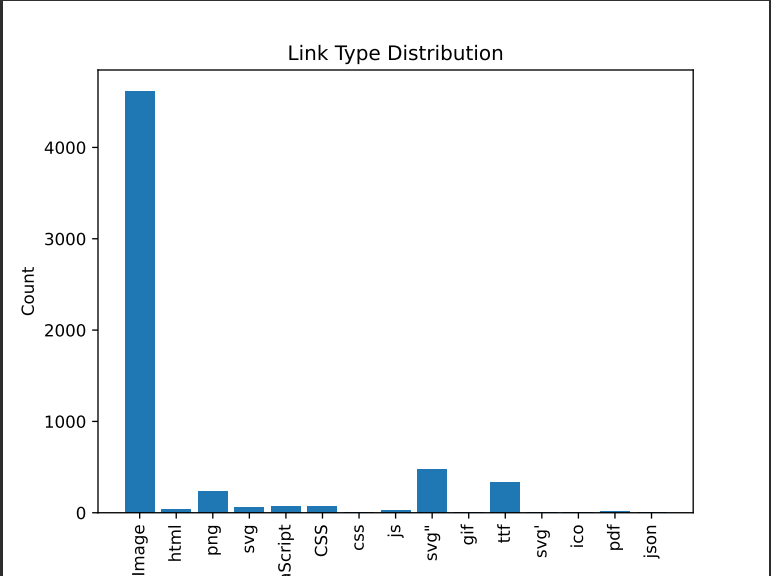
\includegraphics[width=\textwidth]{Screenshot 2023-06-10 123338.png}}
             \caption{Type of Files}
             \label{Type of Files}
         \end{subfigure}
         \hfill
         \begin{subfigure}[b]{0.45\textwidth}
             \centering
             \adjustbox{frame}{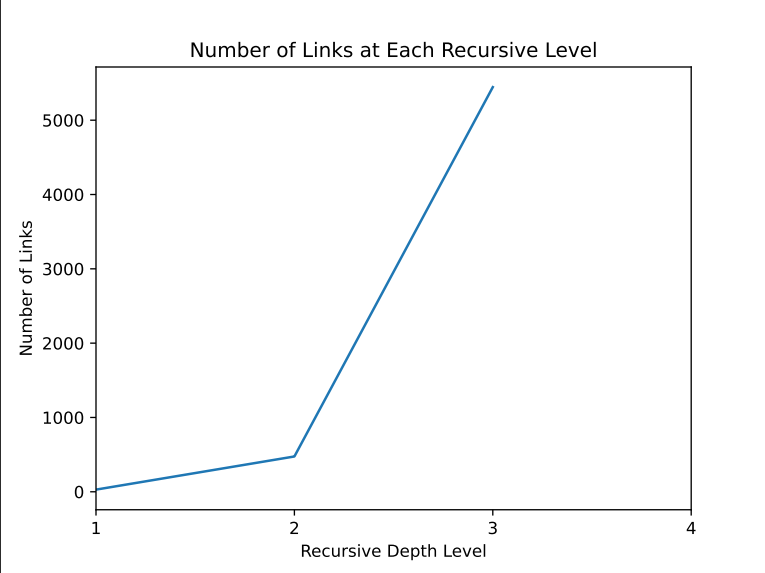
\includegraphics[width=\textwidth]{Screenshot 2023-06-10 123325.png}}
             \caption{Files vs Recursion}
             \label{fig:Example 2}
         \end{subfigure}
            \caption{Sample Output Images}
            \label{fig:three graphs}
\end{figure}
\bibliography{references}

\end{document}